Section 6 works out in detail the user wishes 6.1 – 6.6 mentioned in Section 5, each in a separate subsection. The
user wish itself serves as the title of the subsection (e.g., Register a Good). Each subsection consists of the
following sub-subsections:
\begin{enumerate}
    \item[\textbf{6.n.1}] Rationale/Context
    \item[\textbf{6.n.2}] User story
    \item[\textbf{6.n.3}] Use case
    \begin{itemize}
        \item Frequency of occurrence
        \item Preconditions
        \item Postconditions
        \item Main Success Scenario
        \item Extensions
        \item Other UC-related issues (optional per subsection)
    \end{itemize}
    \item[\textbf{6.n.4}] System Sequence Diagram (SSD)
    \item[\textbf{6.n.5}] Grey box SD (gb-SD)
    \item[\textbf{6.n.6}] White box SDs (wb-SDs)
    \item[\textbf{6.n.7}] Design considerations (optional per subsection)
\end{enumerate}
\newpage

\subsection{Create a ticket}
\subsubsection{Rationale/Context}
In order to travel, every traveller has to buy a ticket. This can be done in two ways, either by going to the office of the Ferry Service or by buying a ticket online through the new system. 
\subsubsection{User story}
As a \textit{traveller}, I want to \textit{buy a ticket}, from a given origin to a given destination.
\subsubsection{Use Case}
\creator{\studentA}
\updater{\studentB}
\secondUpdater{\studentC}

\textbf{Use Case Name:} Create a ticket

\textbf{Scope:} Tickets buying system

\textbf{Level:} User Goal

\textbf{Primary Actor:} Traveller

\textbf{Stakeholders and Interests:} 
\begin{itemize}
\item \textit{Traveller:} Wants to buy a ticket quickly through the website, without having to go to the office.
\item \textit{Seller:} Wants the ticket purchasing process to become automated, thus to have less paperwork and less manual work.
\end{itemize}

\textbf{Preconditions:}
\begin{itemize}
\item -
\end{itemize}

\textbf{Success Guarantee (Postconditions):}
\begin{itemize}
    \item State change: The information of the ticket has been added.
    \item Output: A .pdf file containing the e-ticket shown to the screen and sent to the traveller's email address.
\end{itemize}

\textbf{Main Success Scenario (Basic Flow):}
\begin{enumerate}
\item The User indicates to the System, the wish to buy a ticket.
\item The System sends the User a ticket customisation form.
\item The User fills in the form: the number of passengers, the number of bikes and dogs, the type of ferry, the origin, and the destination.
\item The User sends the System the filled-in ticket selection form.
\item The System checks whether the form is completed correctly (i.e., complete and error-free).
\item The System informs the User about its findings ("Ok" or indicating the gaps and errors found).
\item If the form is not completed correctly, steps 3 - 6 will be repeated.
\item The System sends the User a payment method form with possible payment methods.
\item The User fills in the form: payment method.
\item The User sends the System the filled-in payment method form.
\item The System checks whether the form is completed correctly (i.e., complete).
\item The System informs the User about its findings ("Ok" or indicating the gaps and errors found).
\item If the form is not completed correctly, steps 9 - 12 will be repeated.
\item The System executes a transaction using the given payment method.
\item The System generates a new, unique ticket code.
\item The System stores all the information about the ticket.
\item The System generates an e-ticket and shows it to the screen.
\item The System sends the User an email address input form.
\item The User fills in the form with his email address.
\item The User sends the System the filled-in email input form.
\item The System checks whether the form is completed correctly (i.e., complete and error-free).
\item The System informs the User about its findings ("Ok" or indicating a syntax error in the introduced email address).
\item If the form is not completed correctly, steps 19 - 22 will be repeated.
\item The System sends the ticket the user's email address.
\end{enumerate}
Extensions:
\begin{enumerate}
    \item[6a.1.] If there is more than one bike per person, the System will notify the user.
    \item[] \phantom{x}
    
    \item[13a.1.] If the user has chosen iDEAL in the form at step 9, the System sends the User a form containing the possible banks.
    \item[13a.2.] The User chooses the preferred bank.
    \item[13a.3.] The User sends the System the filled-in payment information form.
    \item[13a.4.] The System checks whether the form is completed correctly (i.e., complete and error-free).
    \item[13a.5.] The System informs the User about its findings ("Ok" or indicating the gaps and errors found).
    \item[13a.6.] If the form is not completed correctly, steps 13a.2 - 13a.5 will be repeated.
    \item[] \phantom{x}
    
    \item[13b.1.] If the user has chosen credit card payment in the form at step 9, the System sends the User a form containing the credit card holder, the credit card expiration date, the credit card number.
    \item[13b.2.] The User fills in: the credit card holder, the credit card expiration date, the credit card number.
    \item[13b.3.] The User sends the System the filled-in payment information form.
    \item[13b.4.] The System checks whether the form is completed correctly (i.e., complete and error-free).
    \item[13b.5.] The System informs the User about its findings ("Ok" or indicating the gaps and errors found).
    \item[13b.6.] If the credit card number and/or expiration date is not valid, the System will inform the User.
    \item[13b.7.] If the form is not completed correctly, steps 13b.2 - 13b.6 will be repeated.
    \item[] \phantom{x}
    
    \item[14a.] If the transaction fails, then the System show the reason of the error to the User and returns him to the payment information form.
\end{enumerate}

\textbf{Technology And Data Variations List:} 
\begin{itemize}
    \item Cardholder name: String with alphabetical characters only
    \item Departure and return date: Date of the form DD/MM/YYYY
    \item Card expiration date: Date of the form MM/YYYY
    \item Number of bikes and dogs: Integer
    \item CVV card code: Three digit number
    \item Destination name, Ferry type, Bank name: String chosen from a list
    \end{itemize}

\textbf{Frequency of Occurrence:} Multiple times a day, every day.

\subsubsection{SSD}
\creator{\studentA}
\updater{\studentB}
\secondUpdater{\studentC}
Considering the previous sub-sections we can create the following SSD model:\\\\
User $\rightarrow$ System: BuyTicket;\hfill /* 1\\
System $\rightarrow$ User: Ticket selection form;\hfill /* 2\\
repeat User $\rightarrow$ User: Fill in the form with: \underline{number of passengers}, \underline{number of bikes},\\ \underline{number of dogs}, \underline{type of ferry}, \underline{destination city};\hfill /* 3\\
\phantom{x}\hspace{7mm} User $\rightarrow$ System: Filled-in Ticket selection form;\hfill /* 4\\
\phantom{x}\hspace{7mm} System $\rightarrow$ System: Check whether the form is completed correctly; \hfill /* 5\\
\phantom{x}\hspace{7mm} System $\rightarrow$ User: "Ok" or the found gaps and errors;\hfill /* 6\\
\phantom{x}\hspace{7mm} if number of bikes greater than the number of people\\
\phantom{x}\hspace{14mm} then System $\rightarrow$ User: "You can only bring one bike per person!"; \hfill /* 6a.1\\
until the form is completed correctly;\hfill /* 7\\
System $\rightarrow$ User: Payment method form;\hfill /* 8\\
repeat User $\rightarrow$ User: Fill in the payment method form with: \underline{payment method};\hfill /* 9\\
\phantom{x}\hspace{7mm} User $\rightarrow$ System: Filled-in payment form;\hfill /* 10\\
\phantom{x}\hspace{7mm} System $\rightarrow$ System: Check whether the form is completed correctly; \hfill /* 11\\
\phantom{x}\hspace{7mm} System $\rightarrow$ User: "Ok" or the found gaps and errors;\hfill /* 12\\
until the form is completed correctly;\hfill /* 13\\
if payment method is iDEAL\\
then System $\rightarrow$ User: Payment form containing the \underline{possible banks};\hfill /* 13a.1\\
\phantom{x}\hspace{7mm} repeat User $\rightarrow$ User: Fill in the bank of choice;\hfill /* 13a.2\\
\phantom{x}\hspace{14mm} User $\rightarrow$ System: Filled-in payment information form;\hfill /* 13a.3\\
\phantom{x}\hspace{14mm} System $\rightarrow$ System: Check whether the form is completed correctly; \hfill /* 13a.4\\
\phantom{x}\hspace{14mm} System $\rightarrow$ User: "Ok" or the found gaps and errors;\hfill /* 13a.5\\
\phantom{x}\hspace{7mm} until the form is completed correctly;\hfill /* 13a.6\\
else\\
\phantom{x}\hspace{7mm} System $\rightarrow$ User: Payment information form;\hfill /* 13b.1\\
\phantom{x}\hspace{7mm} repeat User $\rightarrow$ User: Fill in payment information form with credit card holder, credit card number and credit card expiration date;\hfill /* 13b.2\\
\phantom{x}\hspace{14mm} User $\rightarrow$ System: Filled-in payment information form;\hfill /* 13b.3\\
\phantom{x}\hspace{14mm} System $\rightarrow$ System: Check whether the form is completed correctly; \hfill /* 13b.4\\
\phantom{x}\hspace{14mm} System $\rightarrow$ User: "Ok" or the found gaps and errors;\hfill /* 13b.5\\
\phantom{x}\hspace{14mm} if credit card and/or expiration date not valid\\
\phantom{x}\hspace{21mm} then System $\rightarrow$ User: "Payment information not valid!";\hfill /*13b.6\\
\phantom{x}\hspace{7mm} until the form is completed correctly;\hfill /* 13b.7\\
fi\\
System $\rightarrow$ System: MakeTransaction using the payment credentials or iDeal;\hfill /* 14\\
if transaction failed\\
then System $\rightarrow$ User: Show the reason for transaction failure and restart process;\hfill /* 14a\\
else System $\rightarrow$ System: GenerateUniqueTicketNumber;\hfill /* 15\\
\phantom{x}\hspace{7mm} System $\rightarrow$ System: SaveInformation;\hfill /* 16\\
\phantom{x}\hspace{7mm} System $\rightarrow$ User: Show the generated e-ticket;\hfill /* 17\\
\phantom{x}\hspace{7mm} System $\rightarrow$ User: Email address form; \hfill /* 18\\
\phantom{x}\hspace{7mm} repeat User $\rightarrow$ User: Fill in email address form with email address; \hfill /* 19\\
\phantom{x}\hspace{14mm} User $\rightarrow$ System: Filled-in email address form;\hfill /* 20\\
\phantom{x}\hspace{14mm} System $\rightarrow$ System: Check whether the form is completed correctly; \hfill /* 21\\
\phantom{x}\hspace{14mm} System $\rightarrow$ User: "Ok" or the found gaps and errors in the email address;\hfill /* 22\\
\phantom{x}\hspace{7mm} until the form is completed correctly;\hfill /* 23\\
\phantom{x}\hspace{7mm} System $\rightarrow$ User: Send the generated e-ticket to the user's email; \hfill /* 24\\
fi

\subsubsection{Grey box SD}
\creator{\studentC}
\updater{\studentA}
\begin{figure}[H]
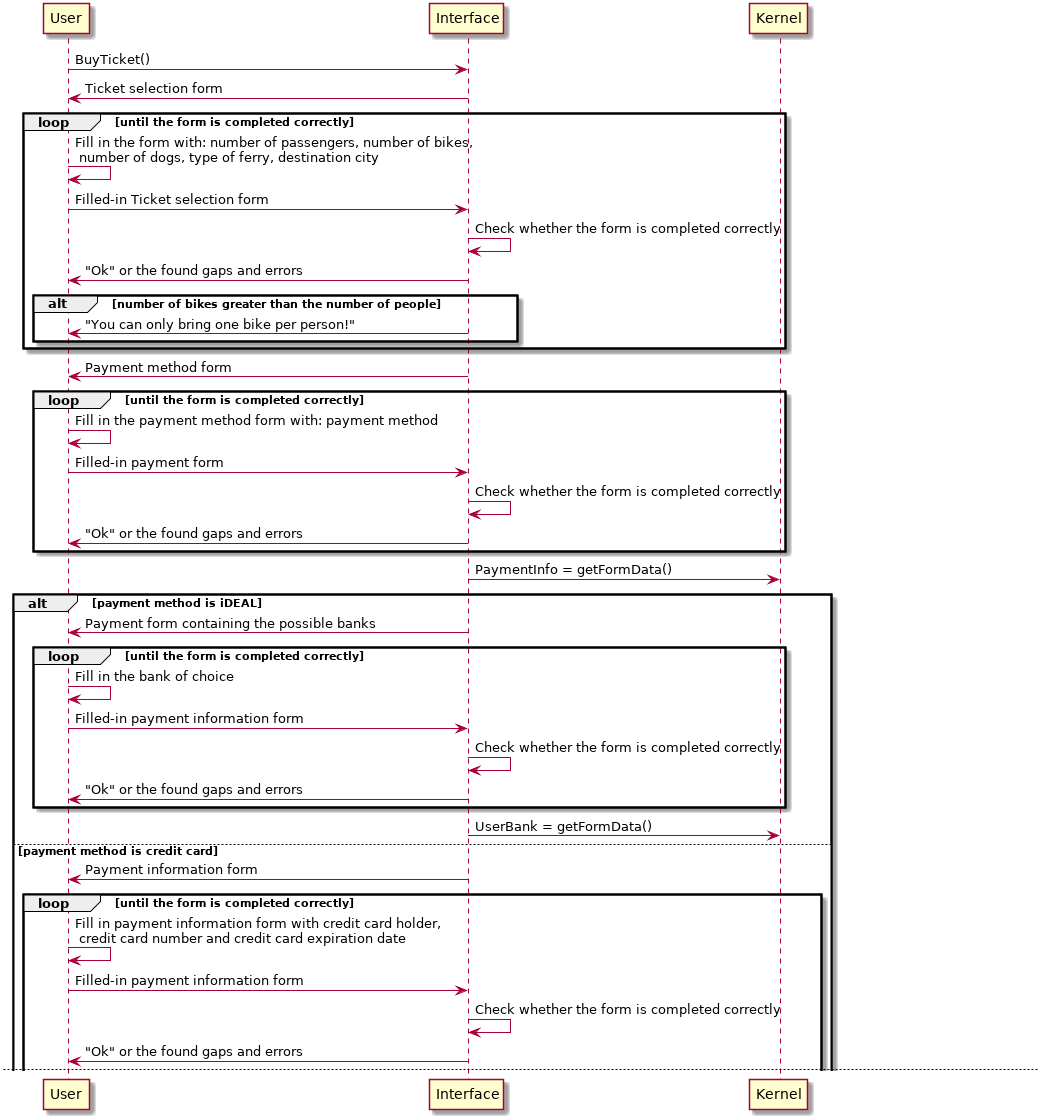
\includegraphics[scale=0.5]{Iteration_3/Files/UC1_gb1.png}
\end{figure}
\begin{figure}[H]
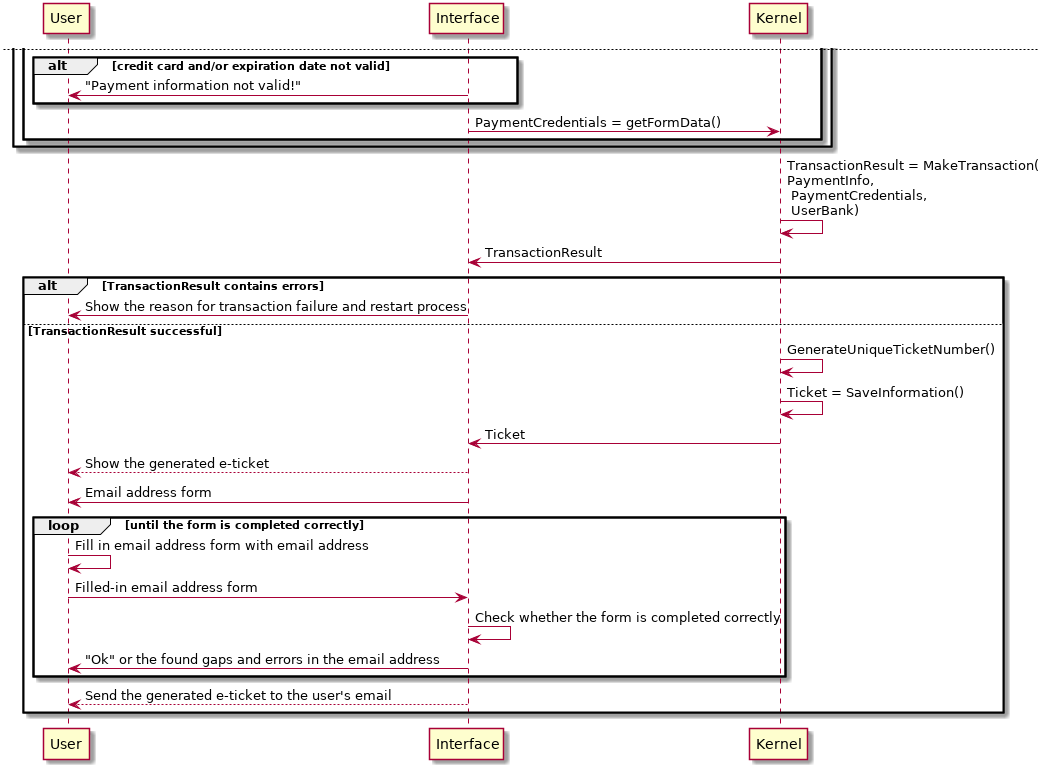
\includegraphics[scale=0.5]{Iteration_3/Files/UC1_gb2.png}
\end{figure}
\iffalse
\begin{lrbox}{\mysavebox}%
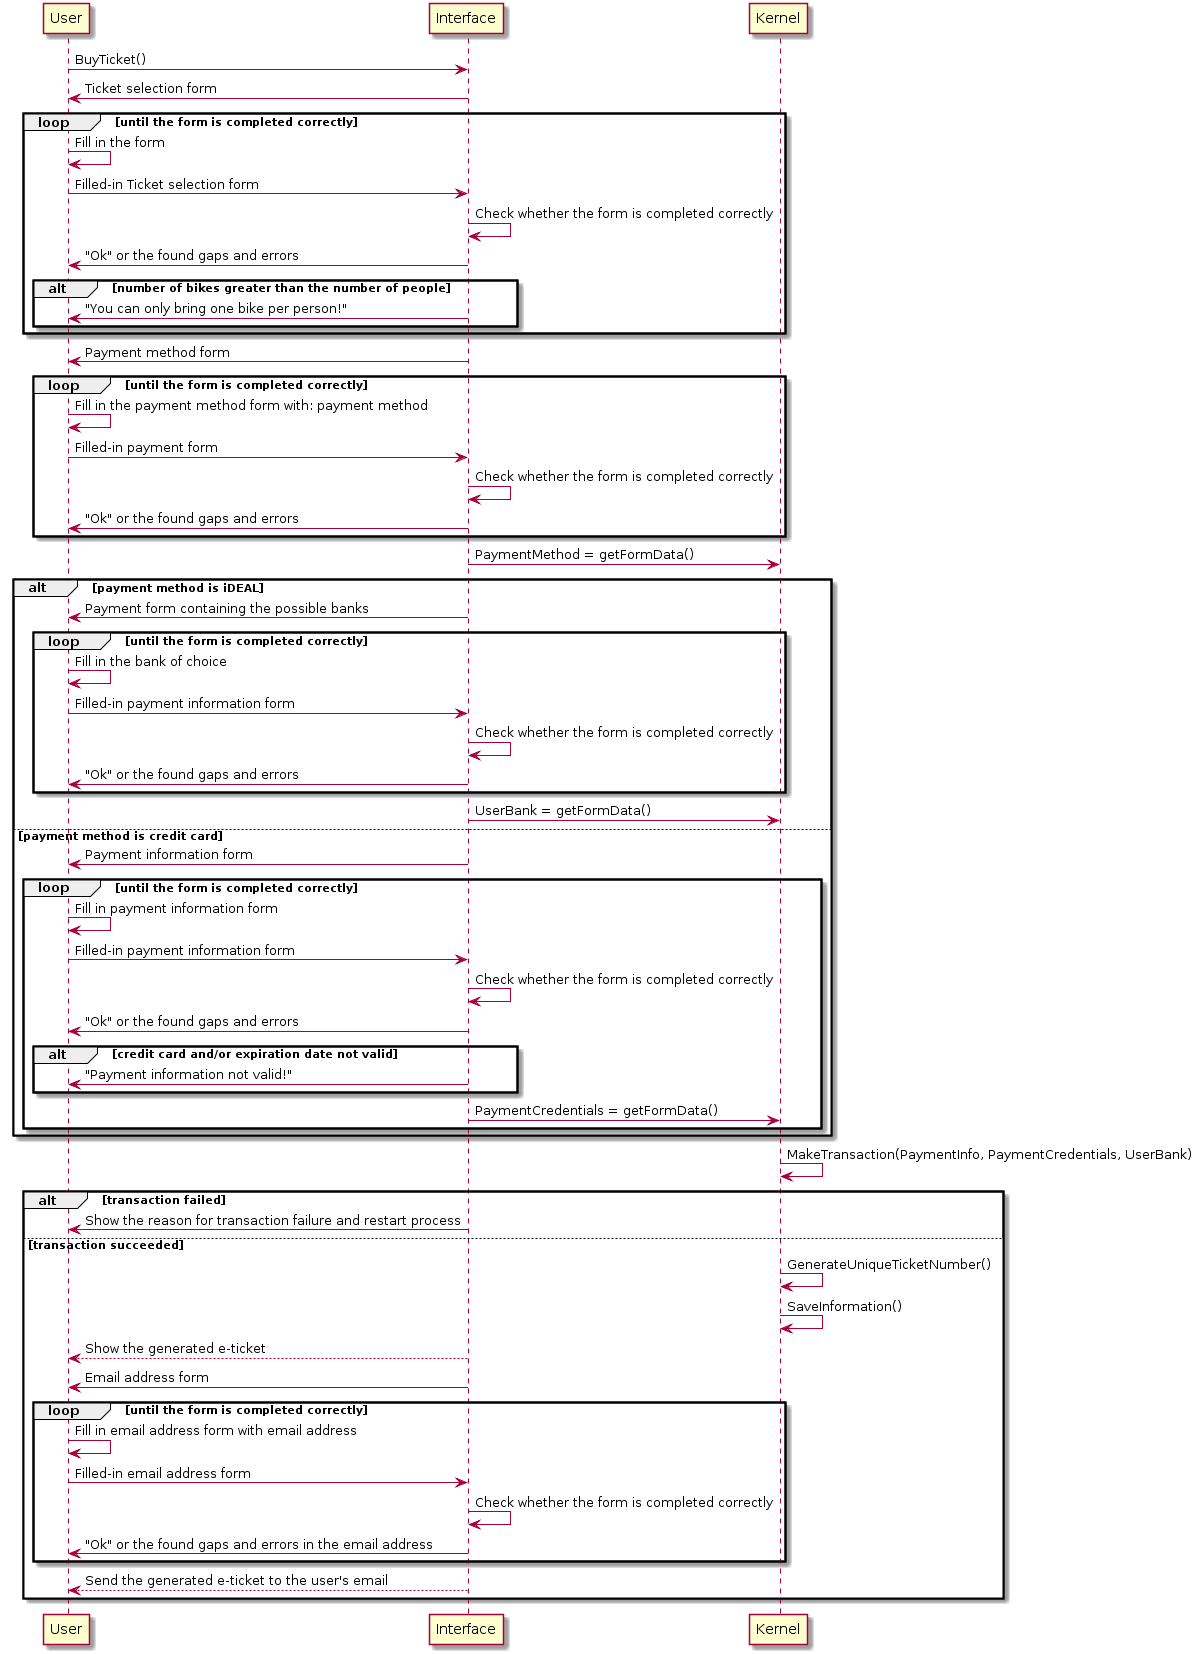
\includegraphics[scale=0.5]{Iteration_3/Files/UC1_gb.png}
\end{lrbox}
\fi

\ifdim\ht\mysavebox>\textheight
    \setlength{\myrest}{\ht\mysavebox}%
    \loop\ifdim\myrest>\textheight
        \newpage\par\noindent
        \clipbox{0 {\myrest-\textheight} 0 {\ht\mysavebox-\myrest}}{\usebox{\mysavebox}}%
        \addtolength{\myrest}{-\textheight}%
    \repeat
    \newpage\par\noindent
    \clipbox{0 0 0 {\ht\mysavebox-\myrest}}{\usebox{\mysavebox}}%
\else
    \usebox{\mysavebox}%
\fi

\subsubsection{White box SD}
\creator{\studentC}
\updater{\studentA}
\begin{figure}[H]
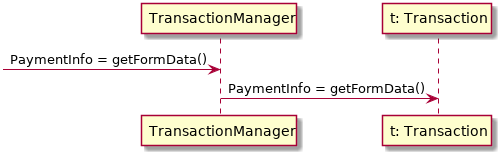
\includegraphics[scale=0.8]{Iteration_3/Files/UC1_wb1.png}
\end{figure}
\begin{figure}[H]
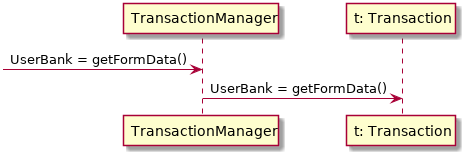
\includegraphics[scale=0.8]{Iteration_3/Files/UC1_wb2.png}
\end{figure}
The previous two white boxes are pretty straightforward, they get the data from the filled-in form and store it in the newly created Transaction object.
\begin{figure}[H]
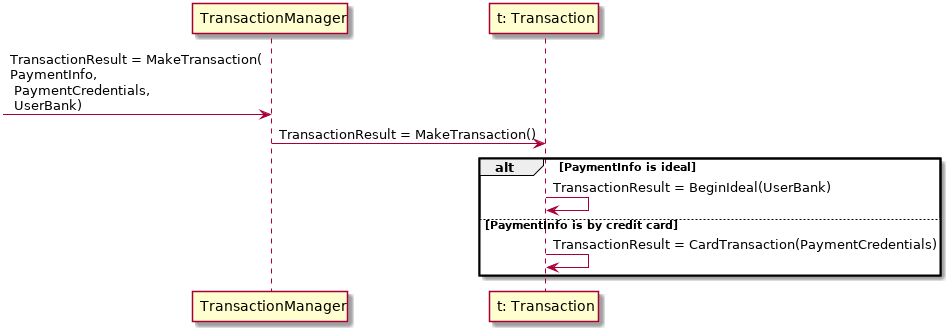
\includegraphics[scale=0.5]{Iteration_3/Files/UC1_wb3.png}
\end{figure}
The Transaction that will be actually executed on the backend depends on the input of the user. If the user chose payment through iDeal, then the service is executed and the response is forwarded back to the object, which in his turn forwards this to the interface. If the chose payment method was credit card, then a simple transaction through a connected microservice (not the scope of our document) is being executed and the result is forwarded back and saved into the object.
\begin{figure}[H]
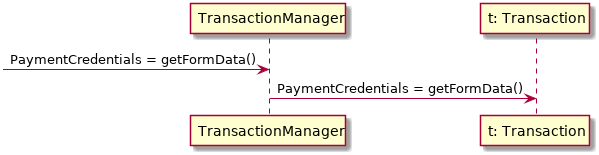
\includegraphics[scale=0.8]{Iteration_3/Files/UC1_wb4.png}
\end{figure}
\begin{figure}[H]
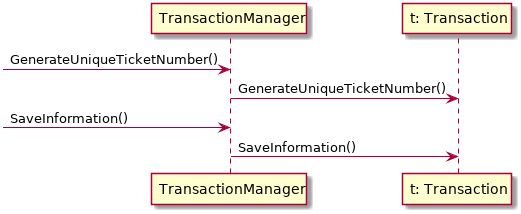
\includegraphics[scale=0.8]{Iteration_3/Files/UC1_wb5.png}
\end{figure}
The previous two white boxes don't need a lot of explanation, functions do as they're named.

\subsubsection{Design Considerations}
\begin{itemize}
    \item For step 12 and 13a.5 from the Main Success Scenario, no possibilities of errors are possible other than not filling-in the form which is already handled.
    \item For the BB-SD, some annotations were shortened so that the final image would be reasonable in size.
\end{itemize}
\newpage

\subsection{Update number of passengers}
\subsubsection{Rationale/Context}
A traveller might want to add a number of passengers, dogs and bikes on their ticket. They can do that until one week before the departure date. If the ticket's information is updated they would have to pay the additional costs.
\subsubsection{User story}
As an employee, I want to update information of a certain ticket.
\subsubsection{Use Case}
\creator{\studentB}
%\updater{Name \textsc{Surname}}
%\secondUpdater{Name \textsc{Surname}}


\textbf{Use Case Name:} Adding extra passengers to a ticket.

\textbf{Scope:} Tickets reservation system

\textbf{Level:} User Goal

\textbf{Primary Actor:}  KOENDES Employee

\textbf{Stakeholders and Interests:} 
\begin{itemize}
\item Stakeholder: KOENDES Employee (wants fast, easy, and accurate retrieval and entry of data).
\item Stakeholder: Traveler (Wants to update the ticket). 
\end{itemize}
\textbf{Preconditions:} 
\begin{itemize}
\item Employee is authenticated
\item Employee is authorised to access this use case.
\item The ticket exists in the system.
\item The departure date is more than a week after the update request.
\end{itemize}

\textbf{Success Guarantee (Postconditions):} 
\begin{itemize}
\item State change: The information has been updated if the departure date of the ticket is at least one week after the date of requesting the update. Otherwise, nothing happens. 
\item Output: "Sorry the update cannot be done due to the late request" if the departure date is within one week; otherwise "The update has been done successfully!".
\end{itemize}

\textbf{Main Success Scenario (Basic Flow):}
\begin{enumerate}
\item The user asks the system to update a ticket.
\item The system sends the user an empty search form for tickets.
\item The user enters the ticket's information provided by traveller such as reservation date, last name or ticket's number.
\item The user sends the filled search form to the system.
\item The system sends back a ticket that matches the search query.
\item The user asks the system to update the selected ticket.
\item The system sends an update form with the actual number of passengers and possible payment methods.
\item The user fills in the number of passengers and the payment method.
\item The user sends the filled update form to the system.
\item The system updates the ticket.
\item The system informs the user with the final result.
\end{enumerate}
Extensions:
\begin{enumerate}
\item[8a] If the payment method can not be processed then the payment should happen before checking-in at the time of travelling.
\end{enumerate}
%\textbf{Alternate Flow:} Alternate Flow

%\textbf{Special Requirements:} Special Requirements

\textbf{Technology And Data Variations List:} 
\begin{itemize}
    \item Last name: String with alphabetical characters only
    \item Reservation date: Date of the form DD/MM/YYYY
    \item Ticket's number: Numerical string
    \end{itemize}
\textbf{Frequency of Occurrence:} 
\begin{itemize}
    \item Regularly.
\end{itemize} 
%\textbf{Open Issues:} Open Issues

\subsubsection{SSD}
\creator{\studentB}
\\
The previous section is necessary for the creation of the SSD:
%\updater{Name \textsc{Surname}}
%\secondUpdater{Name \textsc{Surname}}
Considering the previous sub-sections we can create the following SSD model:\\\\
User $\rightarrow$ System: UpdateTicket;\hfill /* 1\\
System $\rightarrow$ User: Empty tickets search form;\hfill /* 2\\
User $\rightarrow$ User: Adding the provided information from the traveller to the search form;\hfill /* 3\\
User $\rightarrow$ System: Filled-in search form;\hfill /* 4\\
System $\rightarrow$ User: The Ticket that matches the search query;\hfill /* 5\\
User $\rightarrow$ System: UpdateTicket(Ticket);\hfill /* 6\\
System$\rightarrow$ User: An update form;\hfill /* 7\\
User $\rightarrow$ User: Adding the information to the update form;\hfill /* 8\\
User $\rightarrow$ System: Filled-in update form;\hfill /* 9\\
System $\rightarrow$ System: Update Ticket;\hfill /* 10\\
System $\rightarrow$ User: "The ticket has been updated!"\hfill /* 11\\
\iffalse
%\includegraphics[scale=0.9]{UC1}

\subsubsection{Grey box SD}
\creator{Name \textsc{Surname}}
\updater{Name \textsc{Surname}}
%\includegraphics[scale=0.9]{UC1gb.pdf}

\subsubsection{Whte box SD}
\creator{Name \textsc{Surname}}
\updater{Name \textsc{Surname}}

%\includegraphics[scale=0.9]{UC1wb.pdf}
\fi

\subsubsection{Design Considerations}
\newpage

\subsection{UC3}
\subsubsection{Rationale/Context}

Any traveller might want to cancel their reserved trip to one of the islands. Of course, they can do that until one week before the departure date. If the reservation is cancelled they would receive their money back minus the administration fees.

\subsubsection{User story}

As an employee, I want to cancel a certain reservation.

\subsubsection{Use Case}
\creator{\studentC}
\updater{\studentA}
\secondUpdater{\studentB}

\textbf{Use Case Name:} Delete a trip reservation

\textbf{Scope:} Reservations system

\textbf{Level:} User Goal

\textbf{Primary Actor:} KOENDES Employee

\textbf{Stakeholders and Interests:} 
\begin{itemize}
\item \textit{Stakeholder:} KOENDES Employee (Wants an easy and quick process)
\item \textit{Stakeholder:} Traveller (Wants to cancel the reservation)
\end{itemize}

\textbf{Preconditions:} 
\begin{itemize}
\item The reservation exists in the system.
\item The departure date is more than a week after the cancellation request's date.
\item The user is an employee and authorised to make cancellations.
\end{itemize}

\textbf{Success Guarantee (Postconditions):}
\begin{itemize}
\item State change: The reservation has been deleted if the departure date is more than a week after; otherwise it is not deleted and the user gets informed.
\item Output: "Sorry the reservation cannot be cancelled." if the departure date is within one week; otherwise "The reservation has been cancelled!".
\end{itemize}

\textbf{Main Success Scenario (Basic Flow):}
\begin{enumerate}
\item The user asks the system to find a reservation
\item The system sends the user an empty search form for reservations
\item The user enters the reservation's number provided by traveller.
\item The user sends the filled form to the system.
\item The system sends back the reservation that matches the search query.
\item The user asks the system to delete the reservation.
\item The system deletes the reservation if that was possible.
\item The system calculates the refund amount to be the total amount paid minus administration fees.
\item The system sends the refund to the traveller.
\item The system informs the user with the final result.
\end{enumerate}
Extensions:
\begin{enumerate}
\item[7a] The reservation cannot be cancelled if the request is within one week before departure. So the system informs the user that it could not be deleted.
\end{enumerate}
\textbf{Technology And Data Variations List:} 
\begin{itemize}
    \item Last name: String with alphabetical characters only
    \item Reservation date: Date of the form DD/MM/YYYY
    \item Reservation's number: Numerical string
\end{itemize}
\textbf{Frequency of Occurrence:}
\begin{itemize}
    \item Only a few times per month.
\end{itemize}
\subsubsection{SSD}
\creator{\studentC}
\updater{\studentA}
\secondUpdater{\studentB}\\
Considering the previous sub-sections we can create the following SSD model:\\\\
User $\rightarrow$ System: FindReservation;\hfill /* 1\\
System $\rightarrow$ User: Empty reservations search form;\hfill /* 2\\
User $\rightarrow$ User: Inserting (Reservation Number) to the form;\hfill /* 3\\
User $\rightarrow$ System: Filled-in search form;\hfill /* 4\\
System $\rightarrow$ User: The reservation that matches the search query with its (Reservation ID);\hfill /* 5\\
User $\rightarrow$ System: DeleteReservation(Reservation ID);\hfill /* 6\\
if Reservation has a departure date more than 1 week after\\
then System $\rightarrow$ System: Delete Reservation;\hfill /* 7\\
\phantom{x}\hspace{2ex}System $\rightarrow$ System: RefAmount(Reservation ID) = TotalAmount - AdministrationFees;\hfill /* 8\\
\phantom{x}\hspace{2ex}System $\rightarrow$ System: RefundToTraveller(RefAmount);\hfill /* 8\\
\phantom{x}\hspace{2ex}System $\rightarrow$ User: "The reservation has been cancelled!"\hfill /* 9\\
\phantom{x}\hspace{2ex}fi;\\
else System $\rightarrow$ User: "Sorry the reservation cannot be cancelled."\hfill /* 7a\\
fi;\\
%\includegraphics[scale=0.9]{UC1}
\newpage
\subsubsection{Grey box SD}
\creator{\studentB}
\updater{\studentC}
\begin{figure}[H]
    \centering
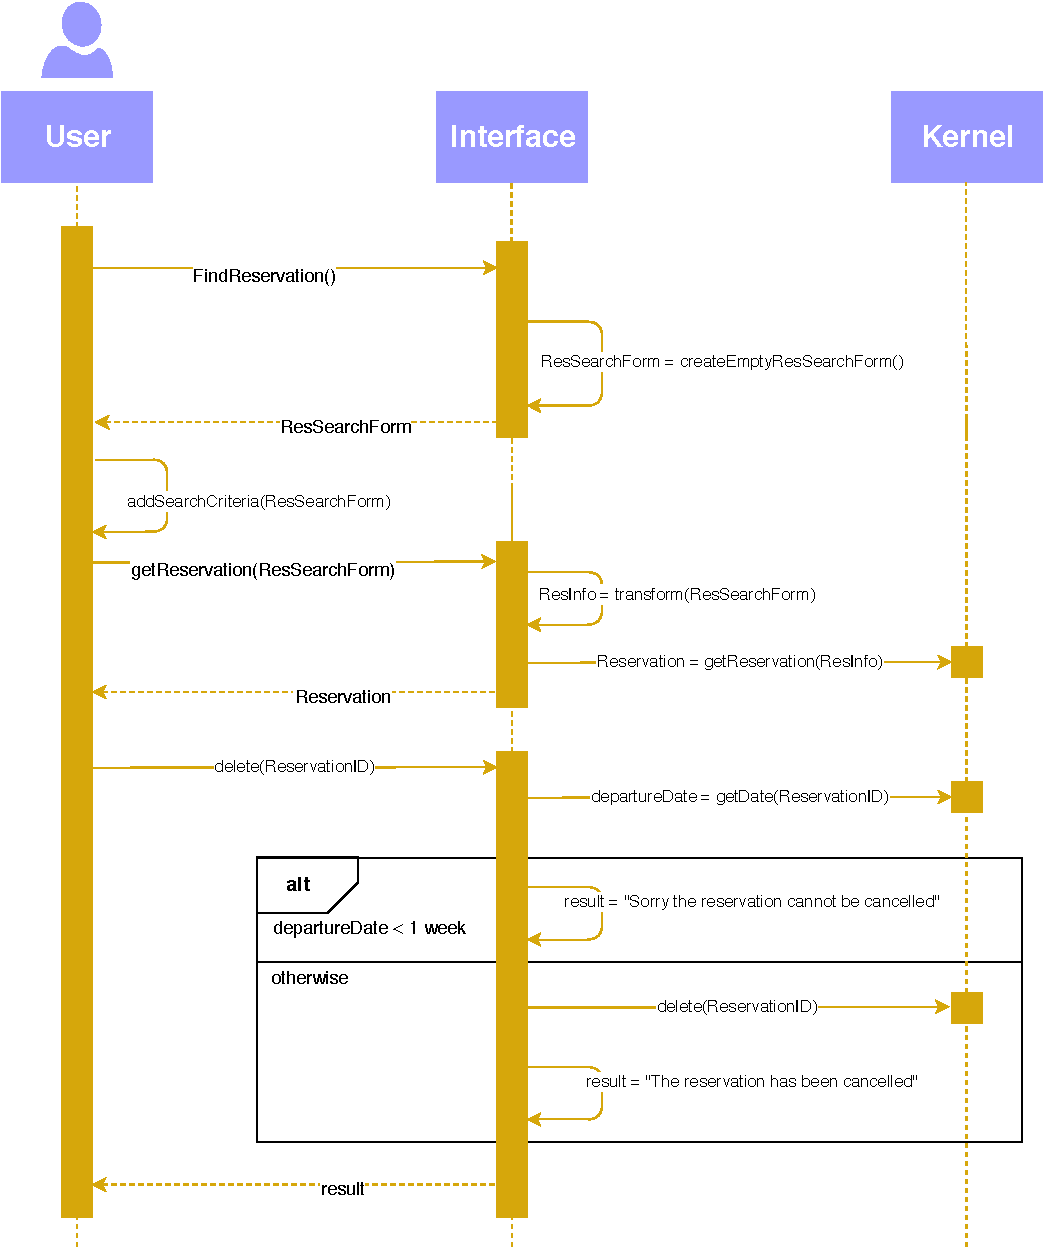
\includegraphics[scale=0.7]{Iteration_3/Files/UC3_gb.pdf}
    \caption{6.3 Grey box}
    \label{fig:6.3 Greybox}
\end{figure}

\subsubsection{White box SD}
\creator{\studentB}
\updater{\studentC}
\begin{figure}[H]
    \centering
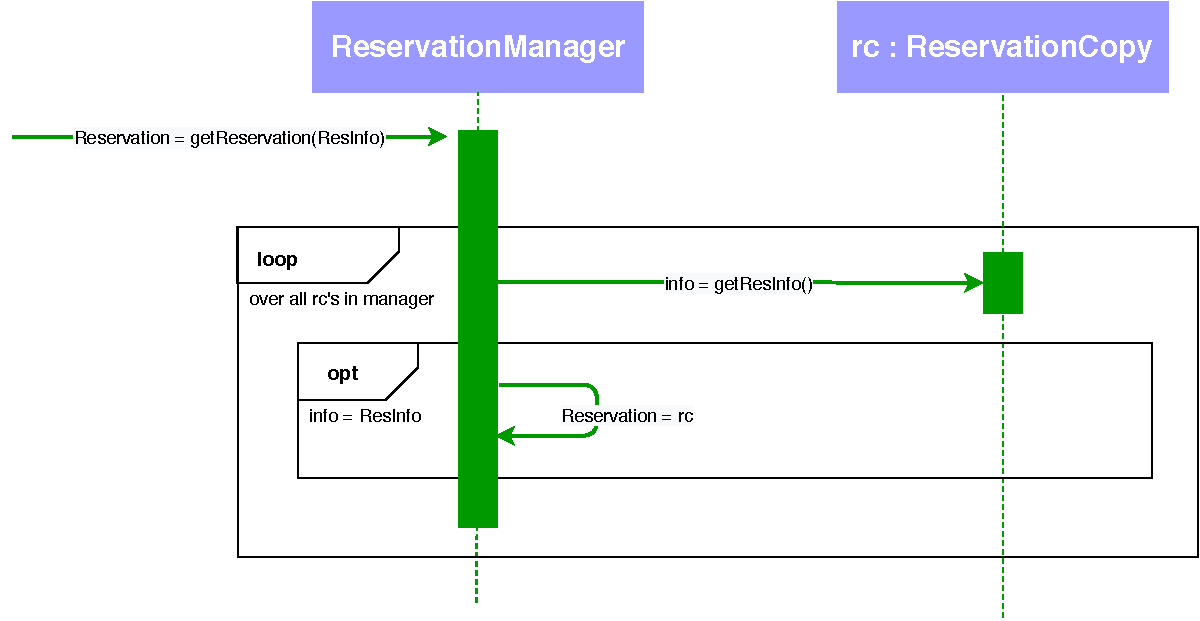
\includegraphics[scale=0.65]{Iteration_3/Files/UC3_wb1.pdf}
\end{figure}
\begin{figure}[H]
    \centering
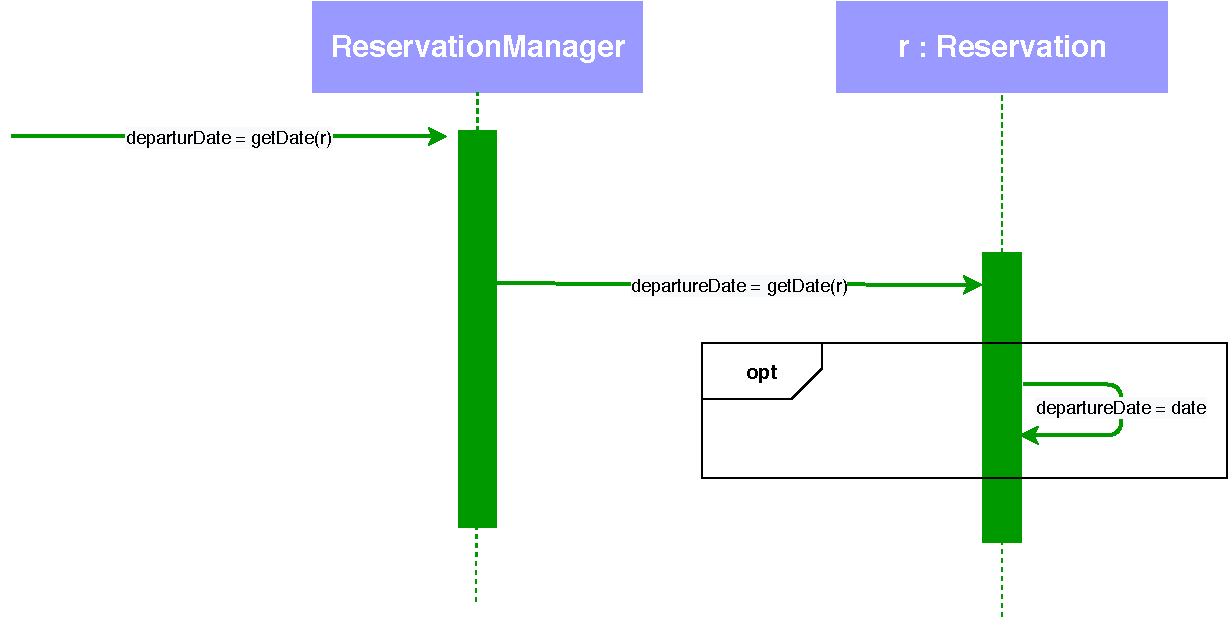
\includegraphics[scale=0.65]{Iteration_3/Files/UC3_wb3.pdf}
\end{figure}
\begin{figure}[H]
    \centering
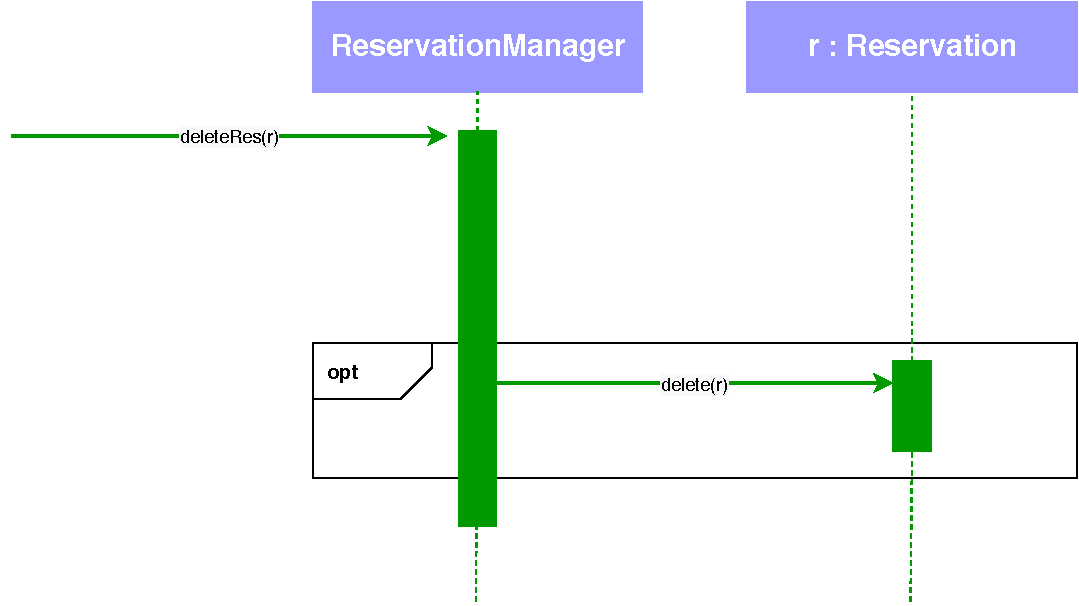
\includegraphics[scale=0.65]{Iteration_3/Files/UC3_wb2.pdf}
\end{figure}

%\includegraphics[scale=0.9]{UC1wb.pdf}

%\subsubsection{Design Considerations}
\newpage